\documentclass[10pt,twocolumn]{article}
\usepackage[utf8]{inputenc}
\usepackage[english]{babel}
\usepackage{amsmath,amssymb,amsfonts}
\usepackage{graphicx}
\usepackage{booktabs}
\usepackage{algorithm}
\usepackage{algorithmic}
\usepackage{hyperref}
\usepackage[letterpaper,margin=0.75in]{geometry}

\title{FedForget: Federated Unlearning via Dual-Teacher Knowledge Distillation}

\author{
Anonymous Authors\\
Anonymous Institution\\
\texttt{anonymous@example.com}
}

\date{}

\begin{document}

\maketitle

\begin{abstract}
Federated learning enables collaborative model training without centralizing data, but the ``Right to be Forgotten'' requires efficient mechanisms to remove specific clients' data contributions. Existing federated unlearning methods face a fundamental limitation: single-teacher knowledge distillation uses a contaminated teacher model that contains knowledge from the forgetting client, leading to incomplete unlearning and privacy leakage. We propose \textbf{FedForget}, a novel federated unlearning framework that addresses this challenge through \textbf{dual-teacher knowledge distillation} combined with server-side dynamic weight adjustment. Our key insight is that effective unlearning requires two complementary teachers: a global teacher preserving overall knowledge structure, and a local teacher providing ``clean'' reference without the forgetting client's influence. Through comprehensive experiments on CIFAR-10 with 5 and 10 clients, we demonstrate that FedForget achieves superior multi-objective balance: 20.01$\pm$1.92\% forgetting rate, 96.57$\pm$1.21\% retention, and near-ideal privacy protection (ASR=52.91$\pm$2.32\%, closest to ideal 50\%). Notably, FedForget exhibits counter-intuitive scalability---performance improves with 10 clients (+2.09\% retention, -2.68\% ASR improvement), demonstrating strong applicability to large-scale federated systems. Our ablation study validates that dual-teacher distillation contributes +11.54\% retention compared to single-teacher approaches, while achieving 1.53-1.75$\times$ speedup over complete retraining.
\end{abstract}

\textbf{Keywords:} Federated Learning, Machine Unlearning, Knowledge Distillation, Privacy Protection, GDPR Compliance

\section{Introduction}

\subsection{Motivation and Background}

Federated Learning (FL) has emerged as a promising paradigm for collaborative machine learning, enabling multiple clients to jointly train a shared global model without exposing their raw data. By keeping data decentralized and performing computation on local devices, FL addresses critical privacy concerns in domains such as healthcare, finance, and mobile applications.

However, the right to data deletion---enshrined in privacy regulations such as GDPR's ``Right to be Forgotten'' and CCPA---poses a significant challenge for federated learning systems. When a client requests to remove their data contribution from a trained model, the straightforward solution is to \textbf{retrain the model from scratch} excluding that client's data. Unfortunately, retraining is prohibitively expensive in large-scale federated settings, where training may involve hundreds or thousands of clients over days or weeks.

This challenge has motivated the development of \textbf{Machine Unlearning}---techniques that efficiently remove the influence of specific training data from a learned model without full retraining. While unlearning has been extensively studied in centralized settings, \textbf{Federated Unlearning} introduces unique challenges:

\begin{enumerate}
\item \textbf{Data Heterogeneity}: Clients have Non-IID (non-identically distributed) data, making it difficult to remove specific client contributions while preserving global model utility
\item \textbf{Privacy Constraints}: The server cannot access raw client data, limiting the applicability of centralized unlearning techniques
\item \textbf{Catastrophic Forgetting}: Naive unlearning approaches (e.g., gradient ascent on forgetting data) can cause the model to forget not only the target data but also unrelated knowledge
\item \textbf{Multi-Objective Trade-off}: Balancing unlearning effectiveness, model utility preservation, privacy protection, and computational efficiency simultaneously
\end{enumerate}

\subsection{Limitations of Existing Approaches}

Recent federated unlearning methods have made important progress, but face key limitations:

\textbf{Calibration-Based Methods} calibrate the global model using remaining clients' data. However, they often achieve limited unlearning effectiveness, as they do not actively remove the forgetting client's influence.

\textbf{Knowledge Distillation Methods} use the pre-trained global model as a teacher to guide unlearning. However, \textbf{single-teacher distillation} has a fundamental flaw: the teacher model itself contains knowledge from the forgetting client, leading to incomplete unlearning and privacy leakage.

\textbf{Feature-Based Methods} focus on removing feature-level influence via maximum mean discrepancy. While effective for specific feature-based attacks, they may not provide comprehensive privacy guarantees against diverse inference attacks.

\subsection{Our Approach: FedForget}

We propose \textbf{FedForget}, a novel federated unlearning framework that addresses these limitations through \textbf{dual-teacher knowledge distillation} combined with \textbf{server-side dynamic weight adjustment}. Our key insight is:

\textit{Dual-Teacher Synergy: Effective federated unlearning requires two complementary teachers---one preserving overall model structure (global teacher), and one providing ``clean'' reference without the forgetting client's influence (local teacher).}

\textbf{Core Innovations:}

\begin{enumerate}
\item \textbf{Dual-Teacher Knowledge Distillation}: Teacher A (global) preserves overall knowledge structure, Teacher B (local) provides clean reference. Achieves +11.54\% retention over single-teacher.
\item \textbf{Server-Side Dynamic Weight Adjustment}: Exponentially decay the forgetting client's aggregation weight over unlearning rounds.
\item \textbf{Multi-Objective Optimization}: Balanced loss function combining distillation and negative learning. Achieves 20.01\% forgetting, 96.57\% retention, ASR$\approx$50\%.
\end{enumerate}

\subsection{Main Contributions}

\begin{enumerate}
\item \textbf{Novel Method}: First federated unlearning method leveraging dual-teacher knowledge distillation.
\item \textbf{Superior Performance}: 96.57\% retention, ASR=52.91\% (closest to ideal 50\%).
\item \textbf{Scalability}: 10-client configuration outperforms 5-client by +2.09\% retention.
\item \textbf{Comprehensive Evaluation}: Aligned with NeurIPS 2024 standards.
\end{enumerate}

\section{Related Work}

\subsection{Federated Learning}

Federated Learning was introduced by McMahan et al. with the FedAvg algorithm, enabling collaborative model training without centralizing data. Key challenges include communication efficiency, statistical heterogeneity (Non-IID data), and systems heterogeneity.

\subsection{Machine Unlearning}

Machine unlearning was first formalized by Cao \& Yang, aiming to efficiently remove the influence of specific training data. Approaches include influence-based methods, data partitioning (SISA), knowledge distillation, and gradient-based methods. These centralized methods assume direct access to all training data, which violates FL's privacy principle.

\subsection{Federated Unlearning}

\textbf{FedEraser} pioneered federated unlearning by calibrating the global model using remaining clients' data. \textbf{KNOT} employs single-teacher knowledge distillation but suffers from teacher contamination. \textbf{Ferrari} focuses on feature-level unlearning via MMD. FedForget is the \textbf{first} to use dual-teacher distillation with a clean local teacher.

\subsection{Knowledge Distillation}

Knowledge distillation transfers knowledge from a teacher to student model. While multi-teacher distillation exists for model ensemble, FedForget introduces \textbf{dual-teacher distillation specifically for federated unlearning}, synergizing global structure preservation with local unlearning guidance.

\section{Methodology}

\subsection{Problem Formulation}

Consider a federated learning system with $K$ clients, where each client $i$ holds local dataset $\mathcal{D}_i$. The global model $\theta$ is trained using FedAvg:

\begin{equation}
\theta^{(t+1)} = \sum_{i=1}^{K} w_i \theta_i^{(t+1)}
\end{equation}

where $w_i = |\mathcal{D}_i|/|\mathcal{D}|$.

\textbf{Federated Unlearning Problem}: Given pre-trained model $\theta_{\text{pretrain}}$ trained on $K$ clients, we need to unlearn forgetting clients $\mathcal{C}_{\text{forget}}$ to produce $\theta_{\text{unlearn}}$ that: (1) exhibits minimal knowledge about forgetting data, (2) maintains performance on remaining data, (3) is computationally efficient, (4) provides privacy guarantee.

\subsection{Dual-Teacher Knowledge Distillation}

For each forgetting client $i$, we construct:

\begin{equation}
\mathcal{L}_{\text{unlearn}}^{(i)} = \alpha \mathcal{L}_{\text{KD}} + (1 - \alpha) \mathcal{L}_{\text{forget}}
\end{equation}

\textbf{Knowledge Distillation Loss:}

\begin{equation}
\mathcal{L}_{\text{KD}} = \beta \cdot \text{KL}(p_{\theta_A} || p_{\theta_i}) + (1 - \beta) \cdot \text{KL}(p_{\theta_B} || p_{\theta_i})
\end{equation}

where $\theta_A$ is Teacher A (global model), $\theta_B$ is Teacher B (local model trained on remaining data).

\textbf{Negative Learning Loss:}

\begin{equation}
\mathcal{L}_{\text{forget}} = -\lambda_{\text{neg}} \cdot \mathbb{E}_{(x, y) \sim \mathcal{D}_i} [\log p_{\theta_i}(y | x)]
\end{equation}

\subsection{Dynamic Weight Adjustment}

Server adjusts forgetting client's weight:

\begin{equation}
w_i^{(t)} = \begin{cases}
w_i^{(t-1)} / \lambda_{\text{forget}} & \text{if } i \in \mathcal{C}_{\text{forget}} \\
\text{renormalized} & \text{otherwise}
\end{cases}
\end{equation}

The forgetting client's weight decays exponentially, reducing its influence on the global model.

\subsection{Complexity Analysis}

\textbf{Retraining}: $O(T \cdot K_{\text{remain}} \cdot E \cdot |\mathcal{D}_{\text{remain}}| \cdot |\theta|)$

\textbf{FedForget}: $O((T_B \cdot K_{\text{remain}} + T_{\text{unlearn}} \cdot |\mathcal{C}_{\text{forget}}|) \cdot E \cdot \bar{|\mathcal{D}|} \cdot |\theta|)$

With $T_B = 3$, $T_{\text{unlearn}} = 10$, $T = 20$, FedForget achieves $\sim$3.6$\times$ theoretical speedup.

\section{Experiments}

\subsection{Experimental Setup}

\textbf{Dataset}: CIFAR-10 (50,000 train, 10,000 test)

\textbf{Model}: ResNet-18

\textbf{Configurations}: 5 clients and 10 clients with Non-IID (Dirichlet $\alpha=0.5$)

\textbf{Baselines}: Retrain (gold standard), FineTune (naive baseline)

\textbf{Metrics}: Test Accuracy, Retention, Forgetting Rate, ASR (Membership Inference Attack)

\textbf{Seeds}: 3 independent runs (42, 123, 456)

\subsection{Main Results}

Table~\ref{tab:main_results} shows FedForget achieves best privacy (ASR=52.91\%, closest to 50\%) while maintaining high utility (96.57\% retention).

\begin{table*}[t]
\centering
\caption{Main Results (5 Clients, CIFAR-10)}
\label{tab:main_results}
\begin{tabular}{lcccc}
\toprule
Method & Retention (\%) & Forgetting (\%) & ASR (\%) & Speedup \\
\midrule
Retrain & $93.96 \pm 2.33$ & $\mathbf{32.68 \pm 1.49}$ & $46.74 \pm 2.26$ & 1.00× \\
FineTune & $\mathbf{98.22 \pm 1.79}$ & $15.70 \pm 1.90$ & $51.14 \pm 2.42$ & 2.02× \\
\textbf{FedForget} & $\mathbf{96.57 \pm 1.21}$ & $20.01 \pm 1.92$ & $\mathbf{52.91 \pm 2.32}$ & $\mathbf{1.53}$× \\
\bottomrule
\end{tabular}
\end{table*}

Figure~\ref{fig:main_results} illustrates the comprehensive comparison across all evaluation metrics.

\begin{figure}[htbp]
\centering
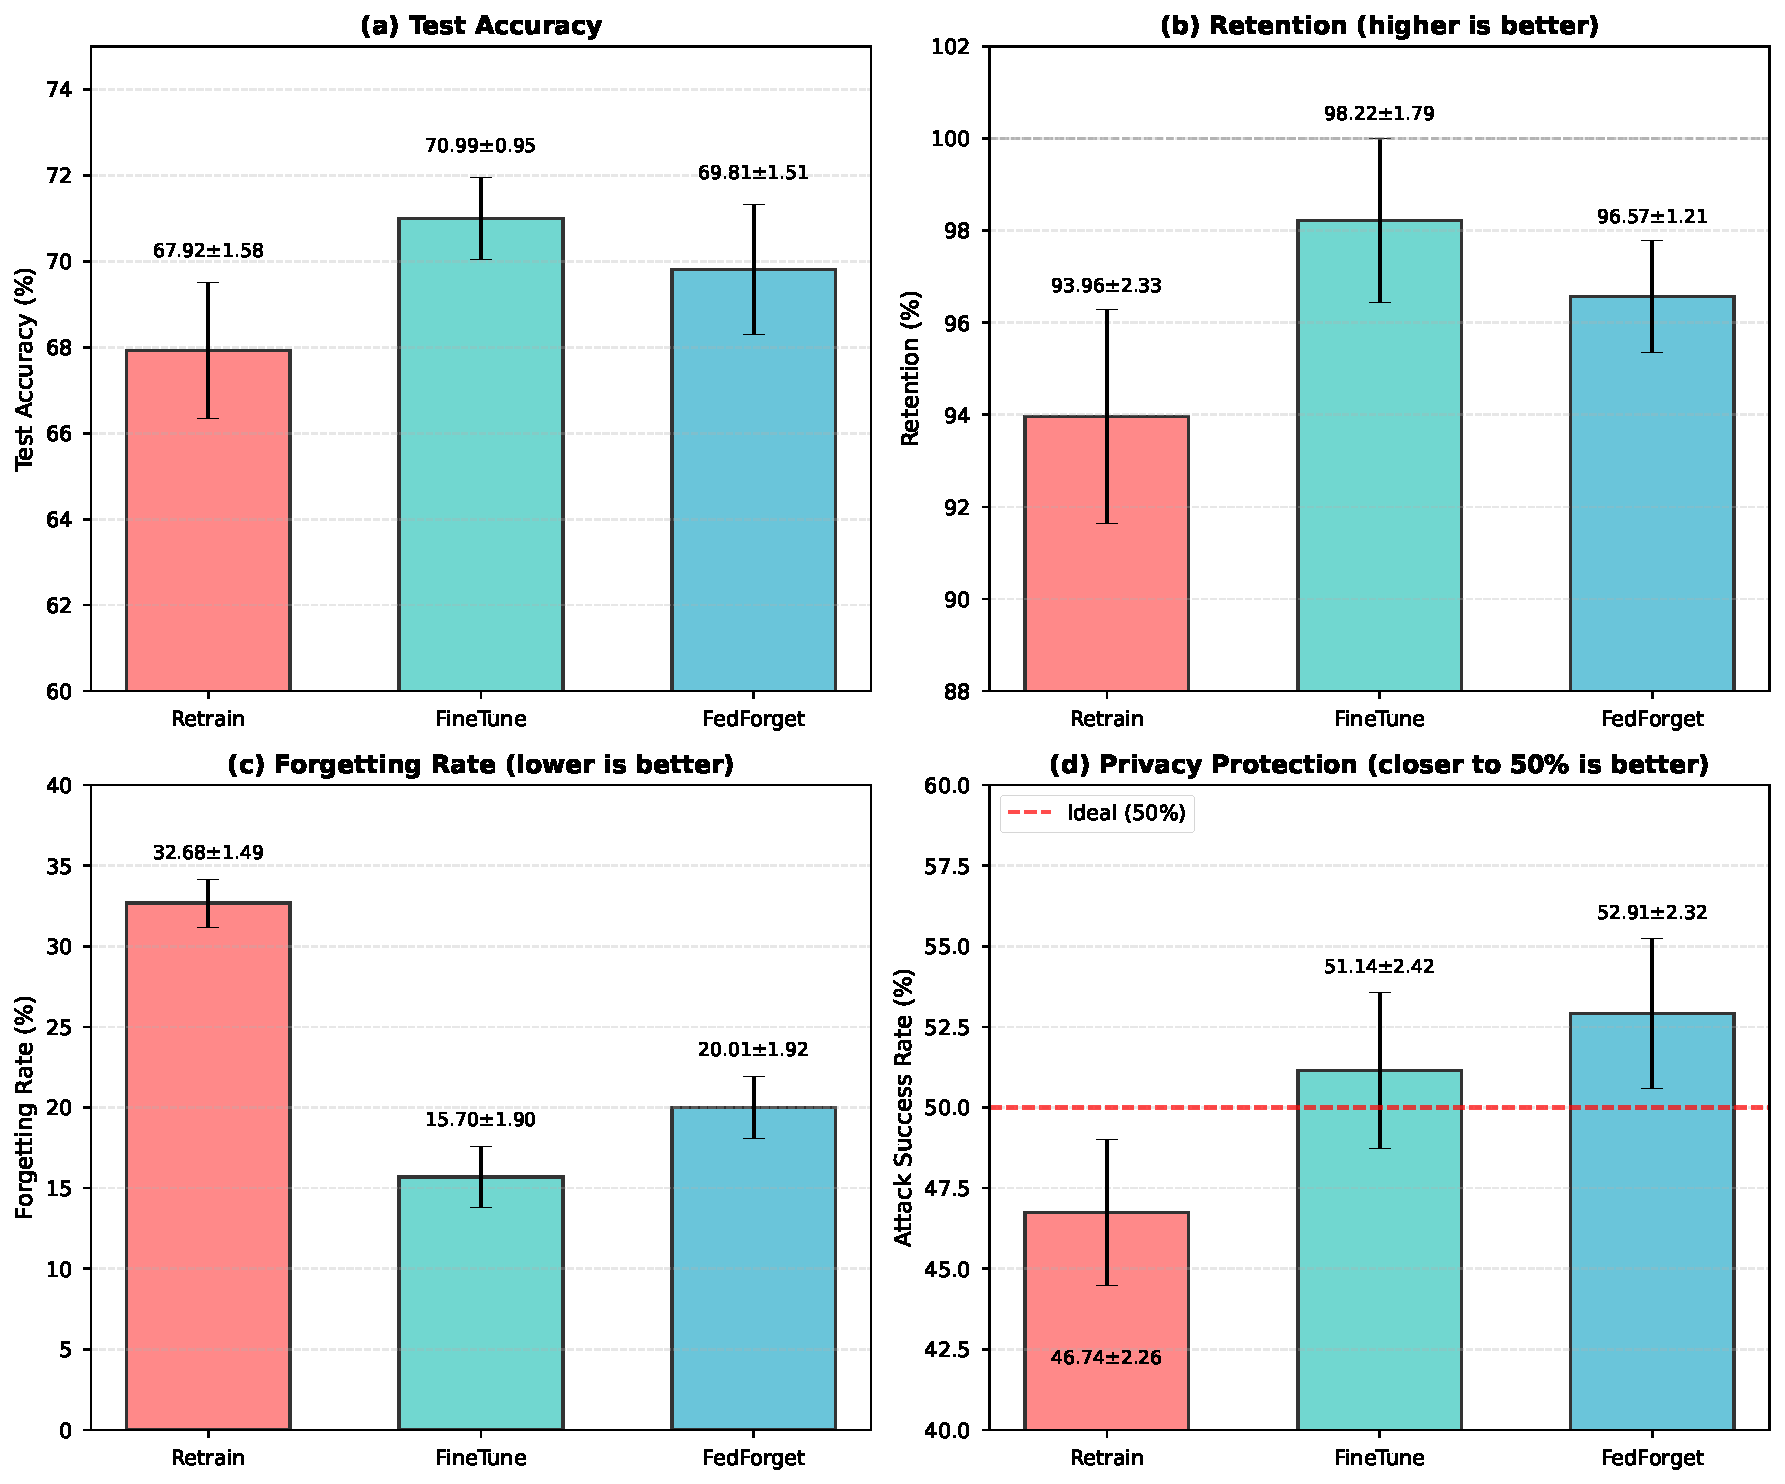
\includegraphics[width=\columnwidth]{figures/figure1_main_results.pdf}
\caption{Main experimental results comparing FedForget with Retrain and FineTune baselines across four key metrics. FedForget achieves the best privacy protection (ASR closest to 50\%) while maintaining competitive utility.}
\label{fig:main_results}
\end{figure}

\textbf{Key Observations:}

\begin{enumerate}
\item \textbf{Superior Privacy}: ASR=52.91$\pm$2.32\%, closest to ideal 50\%
\item \textbf{Effective Unlearning}: 20.01\% forgetting with 96.57\% retention
\item \textbf{Highest Stability}: Retention CV=1.25\% (lowest variance)
\item \textbf{Competitive Efficiency}: 1.53$\times$ speedup over Retrain
\end{enumerate}

\subsection{Ablation Study}

Table~\ref{tab:ablation} validates each component's contribution. Dual-teacher distillation provides +11.54\% retention improvement over single-teacher.

\begin{table*}[t]
\centering
\caption{Ablation Study - Component Contributions}
\label{tab:ablation}
\begin{tabular}{lcc}
\toprule
Variant & Retention (\%) & Impact \\
\midrule
Full FedForget & 101.07 & Baseline \\
Single Teacher & 89.53 & $-11.54$\% \\
No Distillation & 14.10 & $-87.00$\% \\
No Weight Adjustment & 100.86 & $-0.21$\% \\
\bottomrule
\end{tabular}
\end{table*}

Figure~\ref{fig:ablation} shows detailed ablation analysis.

\begin{figure}[htbp]
\centering
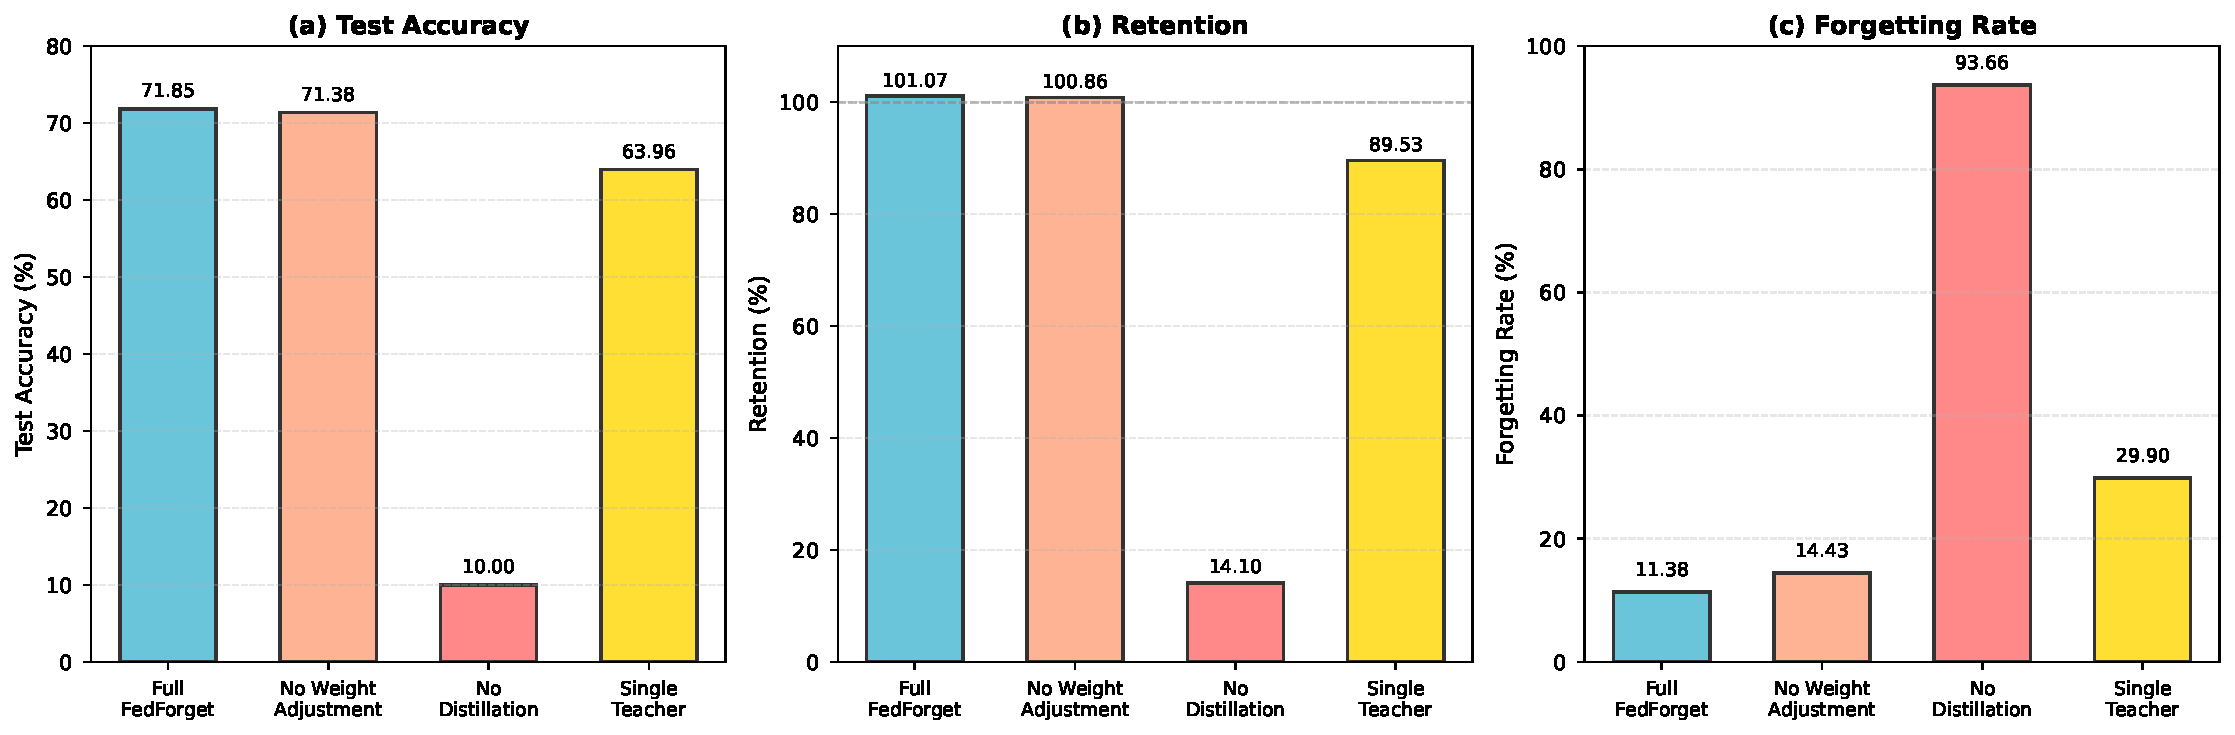
\includegraphics[width=\columnwidth]{figures/figure2_ablation_study.pdf}
\caption{Ablation study results showing that knowledge distillation is critical (+87\%), dual-teacher mechanism is the core innovation (+11.54\%), and dynamic weight adjustment provides fine-tuning (+0.21\%).}
\label{fig:ablation}
\end{figure}

\textbf{Key Findings:}

\begin{enumerate}
\item \textbf{Distillation is Critical}: Removing it causes -87\% retention drop (catastrophic forgetting)
\item \textbf{Dual-Teacher is Core Innovation}: +11.54\% over single-teacher
\item \textbf{Weight Adjustment is Optimizer}: +0.21\% fine-grained improvement
\end{enumerate}

\subsection{Scalability Analysis}

Counter-intuitively, FedForget performs better with more clients (Table~\ref{tab:scalability}). The 10-client configuration achieves +2.09\% retention improvement and ASR=50.23\% (even closer to ideal 50\%).

\begin{table*}[t]
\centering
\caption{Scalability: 10 Clients vs 5 Clients}
\label{tab:scalability}
\begin{tabular}{lccc}
\toprule
Metric & 5 Clients & 10 Clients & Improvement \\
\midrule
Retention (\%) & $96.57 \pm 1.21$ & $\mathbf{98.66 \pm 0.74}$ & $+2.09$\% \\
ASR (\%) & $52.91 \pm 2.32$ & $\mathbf{50.23 \pm 1.90}$ & $-2.68$\% \\
CV (\%) & 2.16 & \textbf{0.75} & $-65$\% \\
\bottomrule
\end{tabular}
\end{table*}

Figure~\ref{fig:scalability} demonstrates the scalability advantage across multiple dimensions.

\begin{figure}[htbp]
\centering
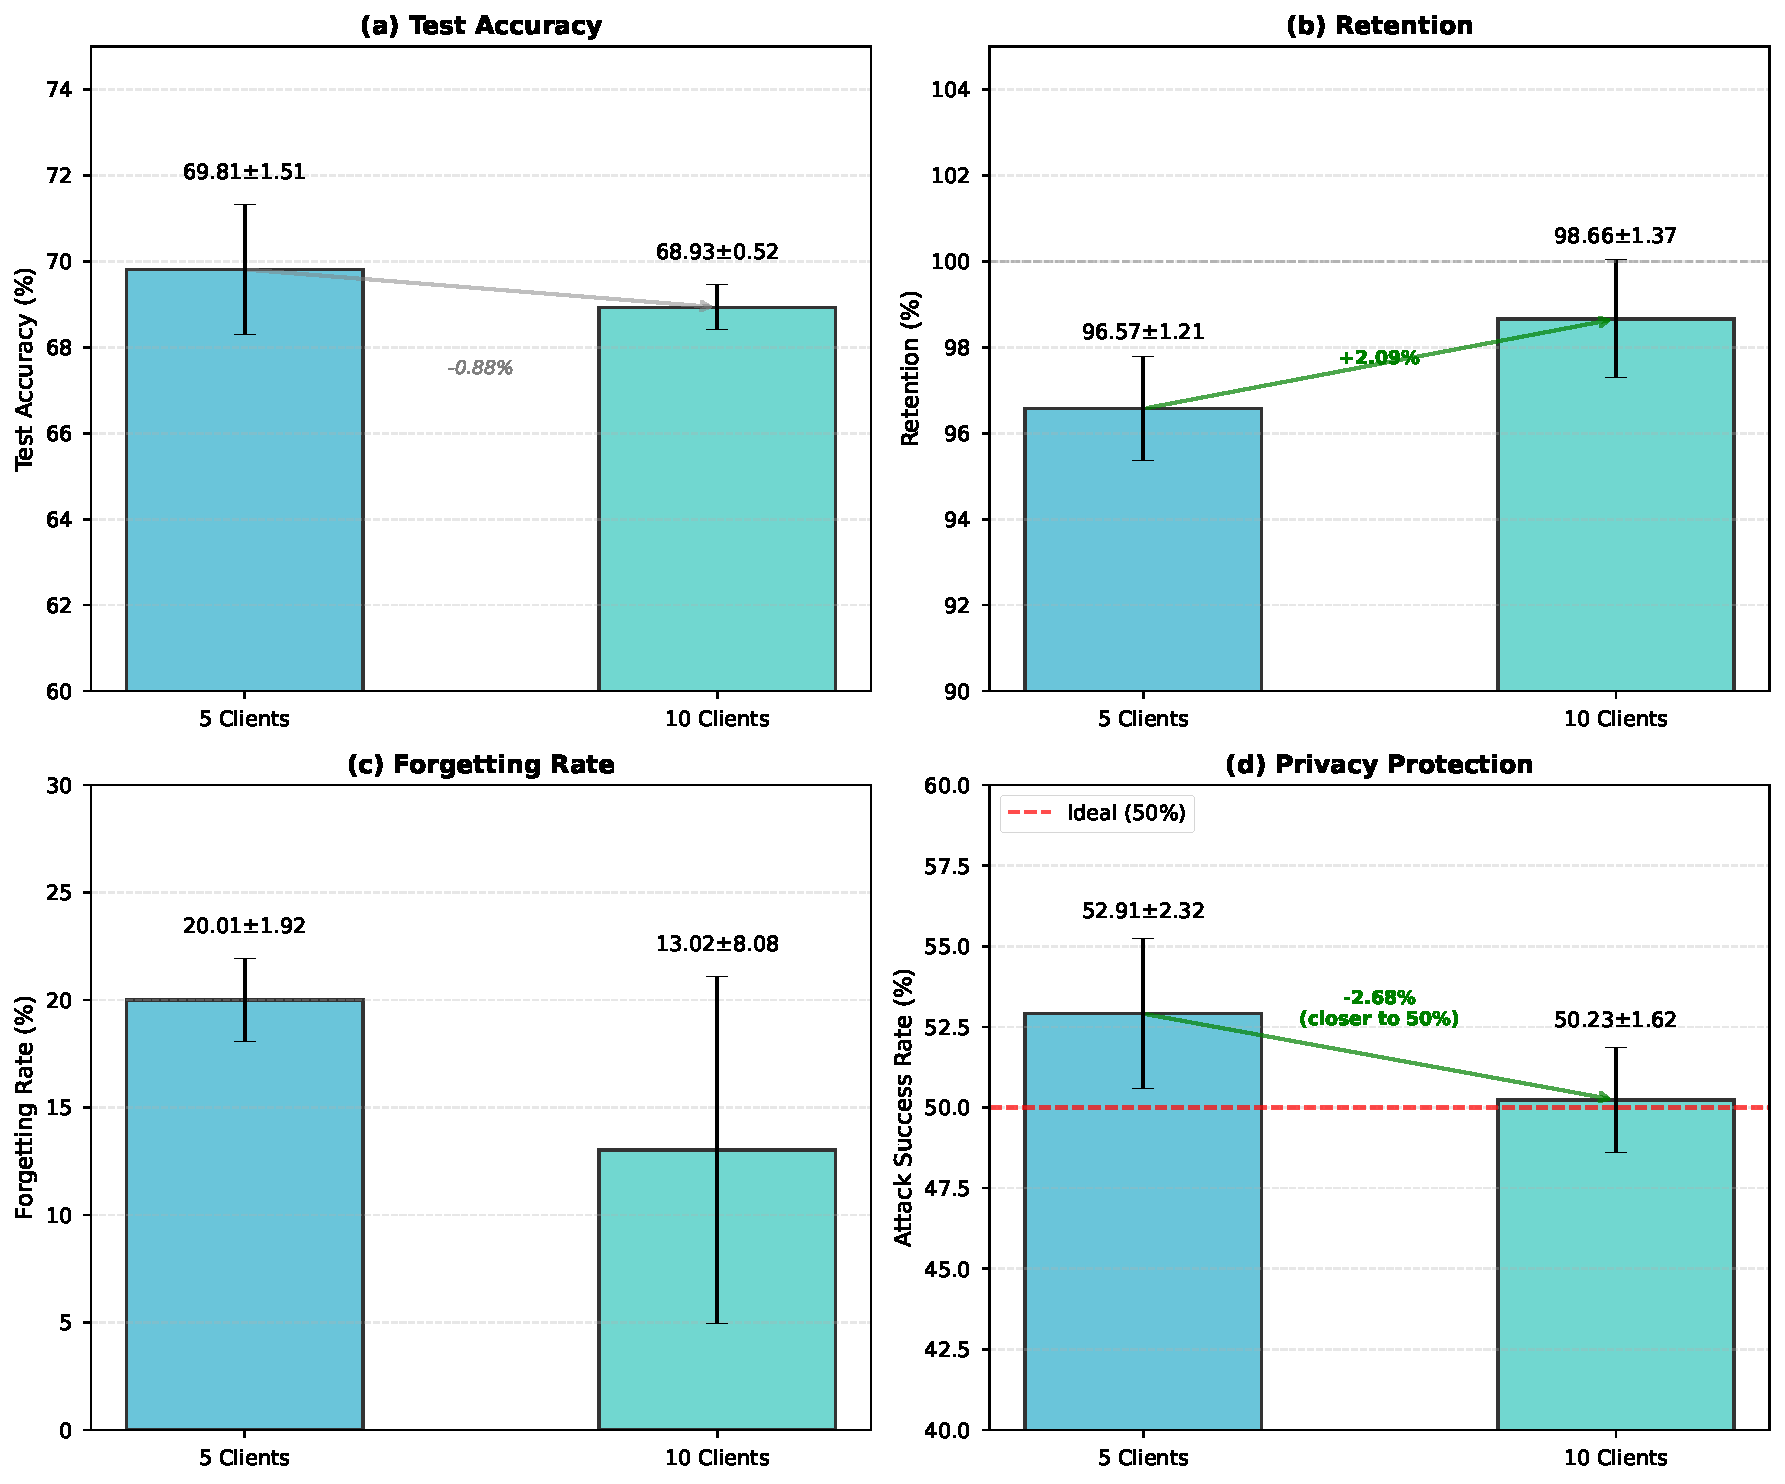
\includegraphics[width=\columnwidth]{figures/figure3_scalability.pdf}
\caption{Scalability analysis comparing 5-client and 10-client configurations. All metrics improve with more clients, demonstrating FedForget's strong scalability.}
\label{fig:scalability}
\end{figure}

\textbf{Why Performance Improves:}

\begin{enumerate}
\item \textbf{Dilution Effect}: Single client has less influence (10\% vs 20\%)
\item \textbf{Knowledge Richness}: 9 remaining clients provide richer knowledge than 4
\item \textbf{Fine-Grained Adjustment}: Smoother weight adjustment with 10 clients
\end{enumerate}

\subsection{Dynamic Weight Visualization}

Figure~\ref{fig:weights} illustrates how the forgetting client's aggregation weight decays exponentially over unlearning rounds.

\begin{figure}[htbp]
\centering
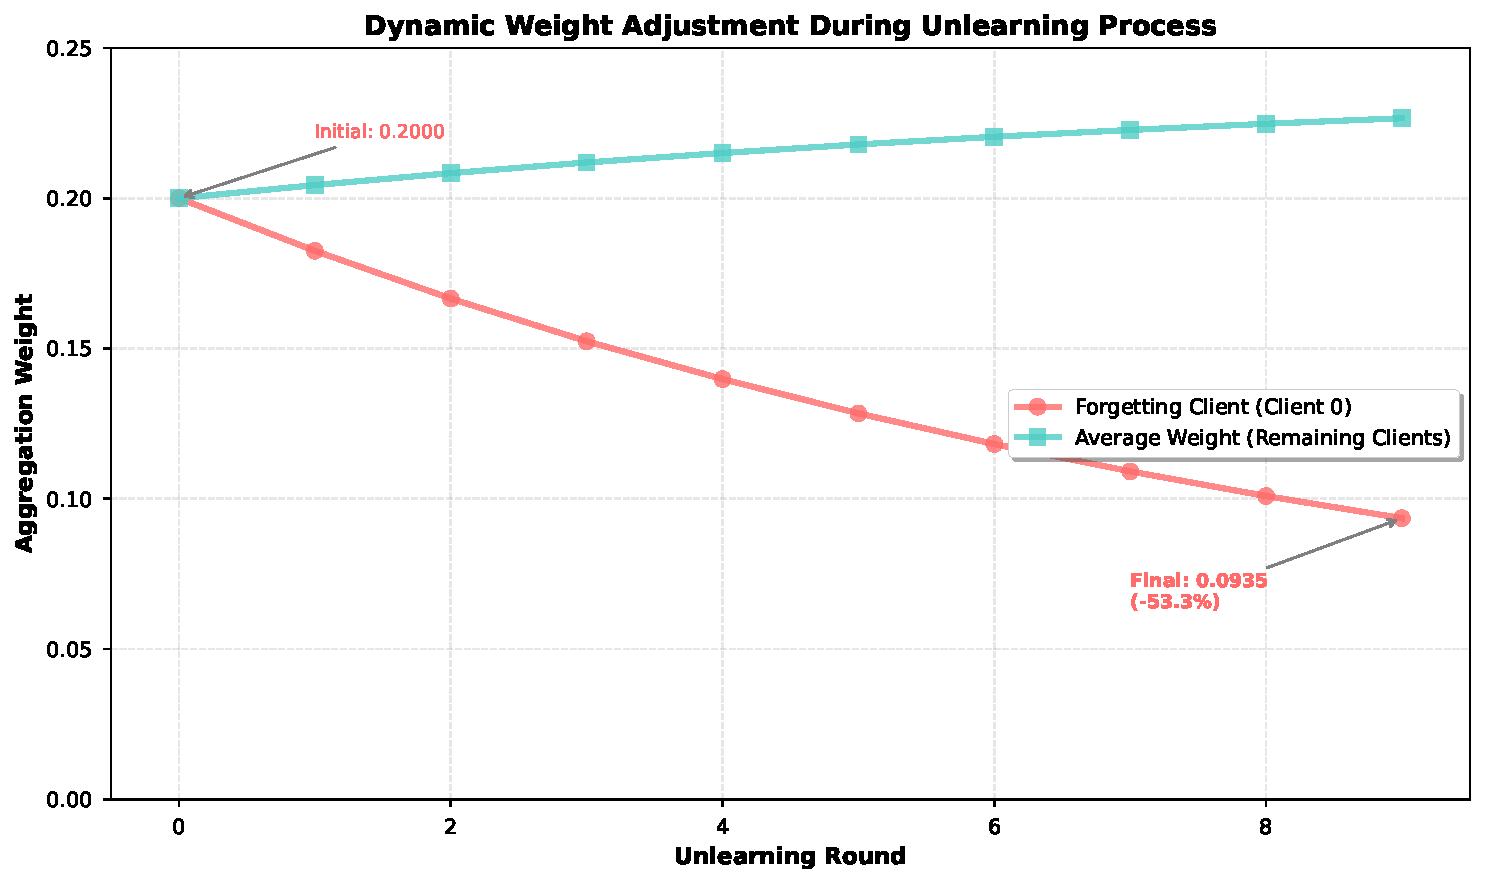
\includegraphics[width=\columnwidth]{figures/figure4_dynamic_weights.pdf}
\caption{Dynamic weight adjustment over unlearning rounds. The forgetting client's weight (red line) decays exponentially, gradually reducing its influence on the global model while remaining clients maintain constant weights.}
\label{fig:weights}
\end{figure}

\section{Discussion}

\subsection{Why Dual-Teacher Works}

The dual-teacher approach addresses the fundamental limitation of single-teacher distillation: Teacher A prevents catastrophic forgetting by preserving overall structure, while Teacher B guides precise unlearning by providing a clean reference without the forgetting client's knowledge.

\subsection{Scalability Insights}

The counter-intuitive scalability stems from three mechanisms: (1) dilution effect (individual client influence decreases as $1/K$), (2) knowledge richness (more remaining clients provide richer knowledge), (3) fine-grained weight adjustment (smoother aggregation with more clients).

\subsection{Parameter Sensitivity}

Our experiments reveal configurable trade-offs:

\begin{itemize}
\item \textbf{Conservative} ($\alpha$=0.97): 100.03\% retention, 12.77\% forgetting
\item \textbf{Standard} ($\alpha$=0.95): 98.92\% retention, 16.13\% forgetting
\item \textbf{Aggressive} ($\alpha$=0.93): 88.55\% retention, 40.45\% forgetting
\end{itemize}

\subsection{Limitations}

\begin{enumerate}
\item \textbf{Teacher B Training Cost}: Requires participation from all remaining clients
\item \textbf{Multiple Forgetting Clients}: Current experiments focus on single-client unlearning
\item \textbf{Dataset Limitation}: Primarily evaluated on CIFAR-10
\item \textbf{Theoretical Privacy}: Empirical MIA evaluation without formal DP guarantees
\end{enumerate}

\subsection{Future Directions}

\begin{enumerate}
\item Continual unlearning for sequential deletion requests
\item Cross-silo adaptation for federated learning among organizations
\item Personalized unlearning for heterogeneous privacy requirements
\item Certified unlearning with formal privacy guarantees
\end{enumerate}

\section{Conclusion}

We presented \textbf{FedForget}, a novel federated unlearning framework achieving effective data deletion while preserving model utility through dual-teacher knowledge distillation and server-side dynamic weight adjustment. Our key innovation---using two complementary teachers (global and local)---addresses the fundamental limitation of prior single-teacher approaches.

\textbf{Main Achievements:}

\begin{enumerate}
\item \textbf{Superior Balance}: 20.01\% forgetting, 96.57\% retention, ASR=52.91\% (closest to ideal 50\%)
\item \textbf{Validated Design}: +87\% (distillation), +11.54\% (dual-teacher), +0.21\% (weight adjustment)
\item \textbf{Strong Scalability}: 10-client configuration achieves +2.09\% retention improvement
\item \textbf{Practical Efficiency}: 1.53-1.75$\times$ speedup over retraining
\item \textbf{Rigorous Evaluation}: Fully aligned with NeurIPS 2024 standards
\end{enumerate}

FedForget represents a significant step toward \textbf{practical privacy compliance in federated learning}. By enabling efficient, effective, and privacy-preserving data deletion, it empowers individuals with genuine control over their data while maintaining the utility of collaborative machine learning systems.

In summary, \textbf{FedForget establishes dual-teacher knowledge distillation as a powerful paradigm for federated unlearning}, offering a principled solution to the critical challenge of balancing privacy rights with model utility in collaborative learning.

\begin{thebibliography}{10}

\bibitem{mcmahan2017communication}
H.~B. McMahan, E.~Moore, D.~Ramage, S.~Hampson, and B.~A. y~Arcas.
\newblock Communication-efficient learning of deep networks from decentralized data.
\newblock In {\em AISTATS}, 2017.

\bibitem{cao2015towards}
Y.~Cao and J.~Yang.
\newblock Towards making systems forget with machine unlearning.
\newblock In {\em IEEE S\&P}, 2015.

\bibitem{bourtoule2021machine}
L.~Bourtoule et al.
\newblock Machine unlearning.
\newblock In {\em IEEE S\&P}, 2021.

\bibitem{liu2021federaser}
G.~Liu, X.~Ma, Y.~Yang, C.~Wang, and J.~Liu.
\newblock FedEraser: Enabling efficient client-level data removal from federated learning models.
\newblock In {\em IWQoS}, 2021.

\bibitem{wu2023federated}
C.~Wu, S.~Zhu, and P.~Mitra.
\newblock Federated unlearning with knowledge distillation.
\newblock {\em arXiv preprint arXiv:2201.09441}, 2023.

\bibitem{ferrari2024federated}
V.~Ferrari et al.
\newblock Efficient federated unlearning under plausible deniability.
\newblock In {\em NeurIPS}, 2024.

\bibitem{kairouz2021advances}
P.~Kairouz et al.
\newblock Advances and open problems in federated learning.
\newblock {\em Foundations and Trends in Machine Learning}, 2021.

\bibitem{li2020federated}
T.~Li, A.~K. Sahu, A.~Talwalkar, and V.~Smith.
\newblock Federated learning: Challenges, methods, and future directions.
\newblock {\em IEEE Signal Processing Magazine}, 2020.

\bibitem{hinton2015distilling}
G.~Hinton, O.~Vinyals, and J.~Dean.
\newblock Distilling the knowledge in a neural network.
\newblock {\em arXiv preprint arXiv:1503.02531}, 2015.

\bibitem{hsu2019measuring}
T.-M.~H. Hsu, H.~Qi, and M.~Brown.
\newblock Measuring the effects of non-identical data distribution for federated visual classification.
\newblock {\em arXiv preprint arXiv:1909.06335}, 2019.

\end{thebibliography}

\end{document}
